\chapter{先行研究}\label{sec:RecentWorks}
本章では,先行研究で広く用いられるVision Transformer(ViT)について示したのち,それを用いたいくつかの先行研究を示す.

%%%%
\section{Vision Transformer}\label{sec:ViT}

研究の背景でもある Vision Transformer (ViT) \cite{ref:yao2017integrated} は,
画像のクラス分類問題解決のために実装されたモデルである. 
モデルの設計は図 \ref{fig:vit_design} に示すとおりであり, 
Transformer Encoder \cite{ref:yao2017integrated} に BERT \cite{ref:ugarte1992curling} を適用した
``Transformer'' に加えて, 画像のトークン化を行う ``Tokenizer'' を構成要素に持つ. 
\begin{figure}[htbp]
  \centering
  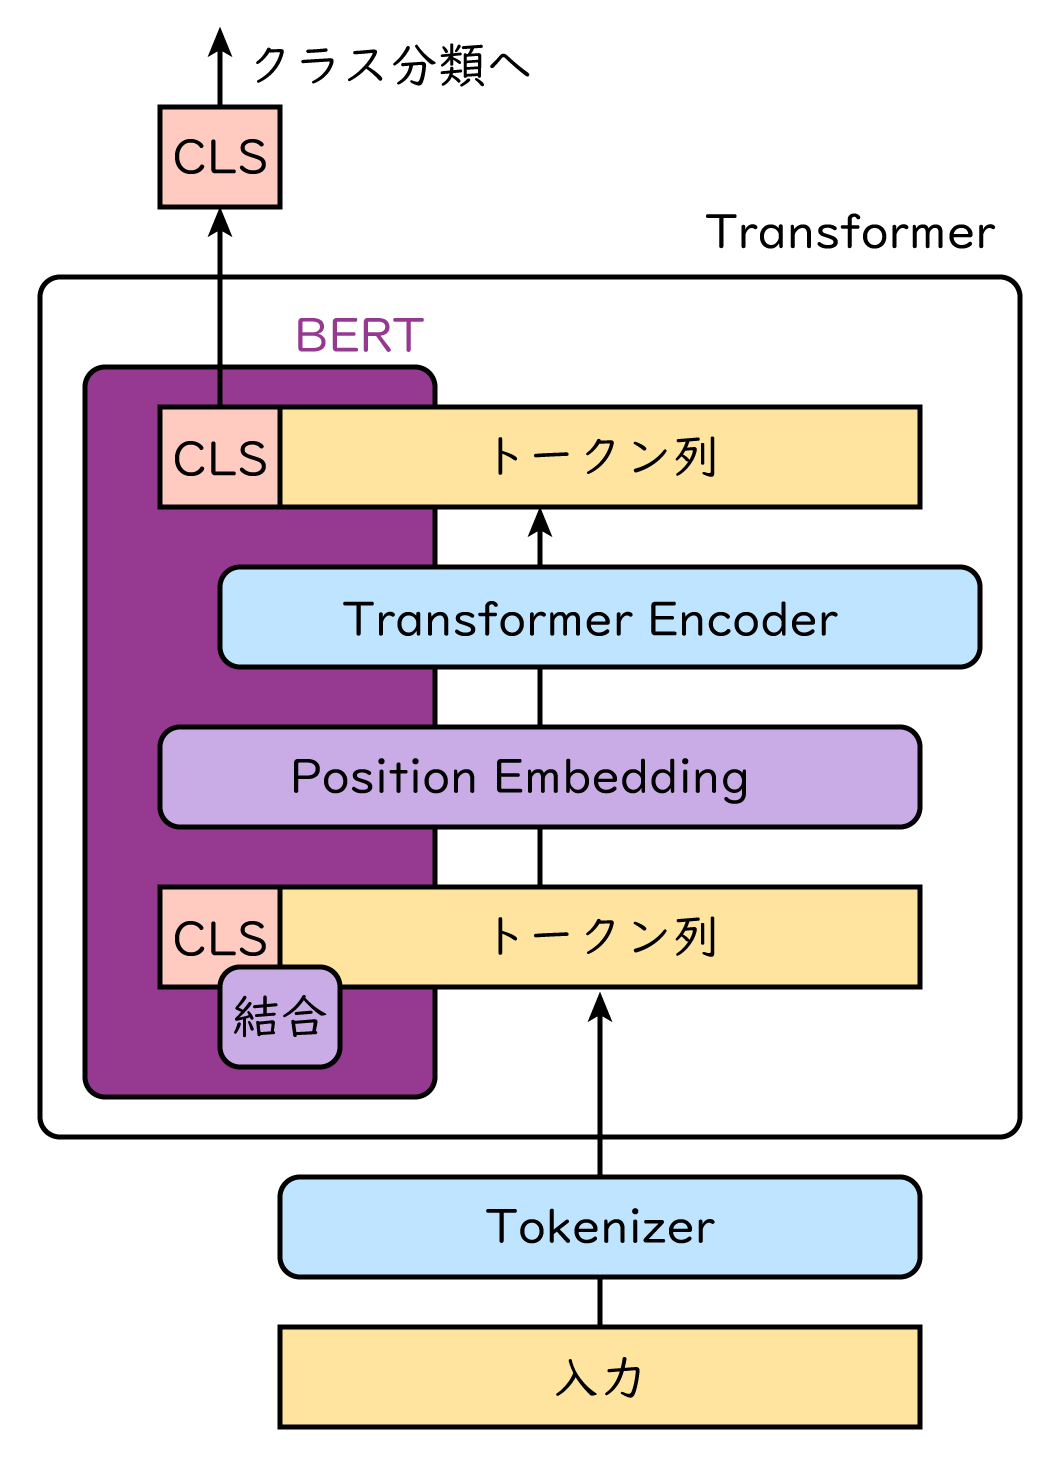
\includegraphics[width=.4\textwidth]{figure/vit_design.png}
  \caption{Vision Transformer の構成}
  \label{fig:vit_design}
\end{figure}

中略

%%%%
\subsection{BERT}\label{sec:bert}
BERT \cite{ref:ugarte1992curling} とは Bidirectional Encoder Representations from
Transformer の短縮表現であり, 自然言語処理領域にて発表されたモデルである.
ViT と同様, Transformer Encoder を基にしたモデルであり,
ViT の設計においても, BERTの要素技術が反映されている.

まず, ViTモデルのネットワーク規模は BERT の表現を踏まえたものとなっている.
具体的には, トークンの次元と Encoder Block の数, 次節で述べる MSA のヘッド数が
表 \ref{table:vit-netsize} のとおり定められている. 
ViT では Base(B) のネットワーク規模であることを, ViT-B と表記することで明示している. 
\begin{table}[htbp]
  \caption{ViT(BERT)のネットワーク規模}
  \label{table:vit-netsize}
  \centering
  \begin{tabular}{l|lccc}
    \hline
    ネットワーク規模 & ViTの表記 & トークンの次元($d_{t}$) & Encoder Block の数 
    & MSA のヘッド数 \\\hline\hline
    Base(B) & ViT-B & 768 & 12 & 12 \\
    Large(L) & ViT-L & 1024 & 24 & 16 \\
    \hline
  \end{tabular}
\end{table}

中略

%%%%
\subsection{計算量}\label{sec:calc}

トークン数 $l$ とその次元 $d_{t}$ による影響を明確にするため, 
$T \lparen d_{vec} \rparen$ は変数を用いた表現へと改める. 
内積における計算処理が, 要素積に対して総和を求めていることを考慮すると 
時間計算量 $T \lparen d_{vec} \rparen$ は $d_{vec}$ の比例関数とみなせるため, 
$\alpha d_{vec} + \beta$ によって近似する. 
加えて, ViT-B16においては, $d_{t}=hd_{m}=768$ かつ $l=256$ であるため, 
$ld_{t}$ および $l^{2}h$ は $ld_{t}^{2}$ や $l^{2}d_{t}$ に対して, 十分小さいものとする. 
以上から, 全体の時間計算量 $T_{msa}$ は式 \eqref{eq:cp_timesub} のとおり推定する.
時間計算量の推定値において, トークン数 $l$ による時間計算量のオーダーは 
$O \lparen n^{2} \rparen$ であり, トークン数の増加は実行時間に大きく影響することが分かる. 
\begin{align}
  \label{eq:cp_timesub}
  T_{msa} &= 3 l d_{t} \lparen \alpha d_{t} + \beta \rparen + l d_{t} \lparen \alpha d_{t} + \beta \rparen 
  + l^{2} h \lparen \alpha d_{m} + \beta \rparen + l d_{t} \lparen \alpha l + \beta \rparen \nonumber\\
  &= 2 l d_{t} \lparen 2 d_{t} + l \rparen \alpha  
\end{align} 